% Options for packages loaded elsewhere
\PassOptionsToPackage{unicode}{hyperref}
\PassOptionsToPackage{hyphens}{url}
%
\documentclass[
]{article}
\usepackage{lmodern}
\usepackage{amssymb,amsmath}
\usepackage{ifxetex,ifluatex}
\ifnum 0\ifxetex 1\fi\ifluatex 1\fi=0 % if pdftex
  \usepackage[T1]{fontenc}
  \usepackage[utf8]{inputenc}
  \usepackage{textcomp} % provide euro and other symbols
\else % if luatex or xetex
  \usepackage{unicode-math}
  \defaultfontfeatures{Scale=MatchLowercase}
  \defaultfontfeatures[\rmfamily]{Ligatures=TeX,Scale=1}
\fi
% Use upquote if available, for straight quotes in verbatim environments
\IfFileExists{upquote.sty}{\usepackage{upquote}}{}
\IfFileExists{microtype.sty}{% use microtype if available
  \usepackage[]{microtype}
  \UseMicrotypeSet[protrusion]{basicmath} % disable protrusion for tt fonts
}{}
\makeatletter
\@ifundefined{KOMAClassName}{% if non-KOMA class
  \IfFileExists{parskip.sty}{%
    \usepackage{parskip}
  }{% else
    \setlength{\parindent}{0pt}
    \setlength{\parskip}{6pt plus 2pt minus 1pt}}
}{% if KOMA class
  \KOMAoptions{parskip=half}}
\makeatother
\usepackage{xcolor}
\IfFileExists{xurl.sty}{\usepackage{xurl}}{} % add URL line breaks if available
\IfFileExists{bookmark.sty}{\usepackage{bookmark}}{\usepackage{hyperref}}
\hypersetup{
  pdftitle={Model Evaluation: Regression},
  pdfauthor={อ.ดร.สิวะโชติ ศรีสุทธิยากร},
  hidelinks,
  pdfcreator={LaTeX via pandoc}}
\urlstyle{same} % disable monospaced font for URLs
\usepackage[margin=1in]{geometry}
\usepackage{color}
\usepackage{fancyvrb}
\newcommand{\VerbBar}{|}
\newcommand{\VERB}{\Verb[commandchars=\\\{\}]}
\DefineVerbatimEnvironment{Highlighting}{Verbatim}{commandchars=\\\{\}}
% Add ',fontsize=\small' for more characters per line
\usepackage{framed}
\definecolor{shadecolor}{RGB}{248,248,248}
\newenvironment{Shaded}{\begin{snugshade}}{\end{snugshade}}
\newcommand{\AlertTok}[1]{\textcolor[rgb]{0.94,0.16,0.16}{#1}}
\newcommand{\AnnotationTok}[1]{\textcolor[rgb]{0.56,0.35,0.01}{\textbf{\textit{#1}}}}
\newcommand{\AttributeTok}[1]{\textcolor[rgb]{0.77,0.63,0.00}{#1}}
\newcommand{\BaseNTok}[1]{\textcolor[rgb]{0.00,0.00,0.81}{#1}}
\newcommand{\BuiltInTok}[1]{#1}
\newcommand{\CharTok}[1]{\textcolor[rgb]{0.31,0.60,0.02}{#1}}
\newcommand{\CommentTok}[1]{\textcolor[rgb]{0.56,0.35,0.01}{\textit{#1}}}
\newcommand{\CommentVarTok}[1]{\textcolor[rgb]{0.56,0.35,0.01}{\textbf{\textit{#1}}}}
\newcommand{\ConstantTok}[1]{\textcolor[rgb]{0.00,0.00,0.00}{#1}}
\newcommand{\ControlFlowTok}[1]{\textcolor[rgb]{0.13,0.29,0.53}{\textbf{#1}}}
\newcommand{\DataTypeTok}[1]{\textcolor[rgb]{0.13,0.29,0.53}{#1}}
\newcommand{\DecValTok}[1]{\textcolor[rgb]{0.00,0.00,0.81}{#1}}
\newcommand{\DocumentationTok}[1]{\textcolor[rgb]{0.56,0.35,0.01}{\textbf{\textit{#1}}}}
\newcommand{\ErrorTok}[1]{\textcolor[rgb]{0.64,0.00,0.00}{\textbf{#1}}}
\newcommand{\ExtensionTok}[1]{#1}
\newcommand{\FloatTok}[1]{\textcolor[rgb]{0.00,0.00,0.81}{#1}}
\newcommand{\FunctionTok}[1]{\textcolor[rgb]{0.00,0.00,0.00}{#1}}
\newcommand{\ImportTok}[1]{#1}
\newcommand{\InformationTok}[1]{\textcolor[rgb]{0.56,0.35,0.01}{\textbf{\textit{#1}}}}
\newcommand{\KeywordTok}[1]{\textcolor[rgb]{0.13,0.29,0.53}{\textbf{#1}}}
\newcommand{\NormalTok}[1]{#1}
\newcommand{\OperatorTok}[1]{\textcolor[rgb]{0.81,0.36,0.00}{\textbf{#1}}}
\newcommand{\OtherTok}[1]{\textcolor[rgb]{0.56,0.35,0.01}{#1}}
\newcommand{\PreprocessorTok}[1]{\textcolor[rgb]{0.56,0.35,0.01}{\textit{#1}}}
\newcommand{\RegionMarkerTok}[1]{#1}
\newcommand{\SpecialCharTok}[1]{\textcolor[rgb]{0.00,0.00,0.00}{#1}}
\newcommand{\SpecialStringTok}[1]{\textcolor[rgb]{0.31,0.60,0.02}{#1}}
\newcommand{\StringTok}[1]{\textcolor[rgb]{0.31,0.60,0.02}{#1}}
\newcommand{\VariableTok}[1]{\textcolor[rgb]{0.00,0.00,0.00}{#1}}
\newcommand{\VerbatimStringTok}[1]{\textcolor[rgb]{0.31,0.60,0.02}{#1}}
\newcommand{\WarningTok}[1]{\textcolor[rgb]{0.56,0.35,0.01}{\textbf{\textit{#1}}}}
\usepackage{graphicx}
\makeatletter
\def\maxwidth{\ifdim\Gin@nat@width>\linewidth\linewidth\else\Gin@nat@width\fi}
\def\maxheight{\ifdim\Gin@nat@height>\textheight\textheight\else\Gin@nat@height\fi}
\makeatother
% Scale images if necessary, so that they will not overflow the page
% margins by default, and it is still possible to overwrite the defaults
% using explicit options in \includegraphics[width, height, ...]{}
\setkeys{Gin}{width=\maxwidth,height=\maxheight,keepaspectratio}
% Set default figure placement to htbp
\makeatletter
\def\fps@figure{htbp}
\makeatother
\setlength{\emergencystretch}{3em} % prevent overfull lines
\providecommand{\tightlist}{%
  \setlength{\itemsep}{0pt}\setlength{\parskip}{0pt}}
\setcounter{secnumdepth}{-\maxdimen} % remove section numbering

\title{Model Evaluation: Regression}
\author{อ.ดร.สิวะโชติ ศรีสุทธิยากร}
\date{9/1/2020}

\begin{document}
\maketitle

\begin{center}\rule{0.5\linewidth}{0.5pt}\end{center}

บทเรียนนี้จะกล่าวถึง cross-validation technique
ที่ใช้สำหรับตรวจสอบประสิทธิภาพของโมเดลการเรียนรู้ที่พัฒนาขึ้น
เนื้อหาในบทเรียนนี้จะกล่าวถึงมโนทัศน์พื้นฐานของการตรวจสอบประสิทธิภาพโมเดลการเรียนรู้
ดัชนีประสิทธิภาพของโมเดล และเทคนิค cross-validation รายละเอียดมีดังนี้

\hypertarget{uxe21uxe42uxe19uxe17uxe31uxe28uxe19uxe4cuxe1euxe37uxe49uxe19uxe10uxe32uxe19}{%
\section{\texorpdfstring{\textbf{มโนทัศน์พื้นฐาน}}{มโนทัศน์พื้นฐาน}}\label{uxe21uxe42uxe19uxe17uxe31uxe28uxe19uxe4cuxe1euxe37uxe49uxe19uxe10uxe32uxe19}}

ปัญหาหนึ่งที่สำคัญในการพัฒนาโมเดลการเรียนรู้ของเครื่องคือปัญหาโมเดลสอดคล้องกับข้อมูลเกินพอดี
(overfitting)
ปํญหาดังกล่าวเกิดขึ้นเมื่อโมเดลการเรียนรู้ที่พัฒนาขึ้นไม่ว่าจะเป็น
classification model หรือ regression model
สามารถเรียนรู้ความสัมพันธ์ระหว่างตัวแปรในชุดข้อมูลฝึกหัดได้ดีมากเกินไปจนทำให้ความสามารถของโมเดลในการทำนายข้อมูลอื่น
ๆ ที่อยู่นอกเหนือจากชุดข้อมูลฝึกหัดมีจำกัดหรือต่ำมากจนเกินไป
ซึ่งทำให้โมเดลการเรียนรู้ที่พัฒนาขึ้นขาดคุณสมบัติความเป็นนัยทั่วไปของโมเดล
(generalizability) วิธีการที่ช่วยลดทอนหรือป้องกันการเกิดปัญหา
overfitting
ของโมเดลคือการพัฒนาโมเดลการเรียนรู้โดยวิเคราะห์ประสิทธิภาพของโมเดลโดยใช้เทคนิค
cross-validation ที่มีการแบ่งข้อมูลที่ผู้วิเคราะห์มีออกเป็นสองส่วน
ส่วนแรกคือ \textbf{ชุดข้อมูลฝึกหัด (training data)} และส่วนที่สองคือ
\textbf{ชุดข้อมูลทดสอบ (testing data)}

ชุดข้อมูลฝึกหัดจะใช้สำหรับเป็นตัวอย่างให้โมเดลการเรียนรู้ของเครื่องต่าง
ๆ
ได้เรียนรู้ความสัมพันธ์ระหว่างตัวแปรและสร้างโมเดลทางคณิตศาสตร์ที่มีความสามารถในการเลียนแบบความสัมพันธ์ในชุดข้อมูลดังกล่าว
ประสิทธิภาพของโมเดลการเรียนรู้ที่คำนวณจากชุดข้อมูลฝึกหัดนี้สามารถใช้สะท้อนระดับความลำเอียง
(bias) ของโมเดลที่พัฒนาขึ้นได้
อย่างไรก็ตามในบางครั้งโมเดลที่มีระดับความลำเอียงต่ำมาก ๆ
ก็ไม่ใช่โมเดลที่ดีเสมอไป
ทั้งนี้เป็นเพราะโมเดลดังกล่าวมีความสอดคล้องกับข้อมูลในชุดข้อมูลฝึกหัดมากจนเกินไปจนทำให้ไม่สามารถนำไปทำนายค่าสังเกตอื่นที่อยู่นอกเหนือชุดข้อมูลฝึกหัดได้
การตรวจสอบประสิทธิภาพของโมเดลโดยใช้ชุดข้อมูลทดสอบจึงมีความจำเป็น
เนื่องจากข้อมูลในชุดข้อมูลทดสอบนี้เป็นข้อมูลที่โมเดลที่พัฒนาขึ้นยังไม่เคยเรียนรู้มาก่อน
ประสิทธิภาพที่คำนวณได้จากชุดข้อมูลทดสอบนี้จึงสะท้อนคุณสมบัติของโมเดลในด้านความเป็นนัยทั่วไปในการทำนาย

\hypertarget{uxe14uxe31uxe0auxe19uxe35uxe27uxe31uxe14uxe1buxe23uxe30uxe2auxe34uxe17uxe18uxe34uxe20uxe32uxe1euxe02uxe2duxe07uxe42uxe21uxe40uxe14uxe25-model-performance-metric}{%
\section{\texorpdfstring{\textbf{ดัชนีวัดประสิทธิภาพของโมเดล (model
performance
metric)}}{ดัชนีวัดประสิทธิภาพของโมเดล (model performance metric)}}\label{uxe14uxe31uxe0auxe19uxe35uxe27uxe31uxe14uxe1buxe23uxe30uxe2auxe34uxe17uxe18uxe34uxe20uxe32uxe1euxe02uxe2duxe07uxe42uxe21uxe40uxe14uxe25-model-performance-metric}}

บทเรียนนี้จะกล่าวถึงสถิติ 3
ตัวที่มักนิยมใช้เป็นดัชนีวัดประสิทธิภาพในการทำนายของโมเดล ได้แก่

\begin{enumerate}
\def\labelenumi{\arabic{enumi}.}
\item
  \textbf{สัมประสิทธิ์การตัดสินใจ (coefficient of determination:
  \(R^2\))}
  มีค่าเท่ากับกำลังสองของสัมประสิทธิ์สหสัมพันธ์ระหว่างค่าทำนายกับค่าจริง
  ทำให้มีค่าที่เป็นไปได้อยู่ในช่วง \([0,1]\)
  ซึ่งมีความหมายเป็นร้อยละของปริมาณความผันแปรที่มีร่วมกันระหว่างค่าทำนายที่ได้จากโมเดลกับค่าจริง
  โมเดลที่มีค่า \(R^2\) เข้าใกล้ 1 แสดงว่ามีประสิทธิภาพในการทำนายสูง
\item
  \textbf{รากที่สองของความคลาดเคลื่อนกำลังสอง (root mean squares error:
  \(RMSE\))} มีสูตรการคำนวณดังนี้
\end{enumerate}

\[RMSE=\sqrt{\frac{\sum_{i=1}^n(y_i-\hat{y}_i)^2}{n}}\] เมื่อ \(y_i\)
คือค่าสังเกตจริงในชุดข้อมูลทดสอบ, \(\hat{y}_i\)
คือค่าทำนายของค่าสังเกตในชุดข้อมูลทดสอบที่ได้จากโมเดลการเรียนรู้ และ
\(n\) คือขนาดของชุดข้อมูลทดสอบ ดัชนี \(RMSE\)
สะท้อนปริมาณความคลาดเคลื่อนในการทำนายของโมเดลโดยเฉลี่ย โมเดลที่มีค่า
\(RMSE\) ต่ำแสดงว่ามีประสิทธิภาพในการทำนายสูง

\begin{enumerate}
\def\labelenumi{\arabic{enumi}.}
\setcounter{enumi}{2}
\tightlist
\item
  \textbf{ส่วนเบี่ยงเบนเฉลี่ยของความคลาดเคลื่อน (absolute mean error:
  \(MAE\))} มีสูตรการคำนวณดังนี้
\end{enumerate}

\[MAE=\frac{\sum_{i=1}^n|y_i-\hat{y}_i|}{n}\] จากสูตรข้างต้นจะเห็นว่า
\(MAE\) มีความหมายเหมือนกับ \(RMSE\)
แต่มีการใช้ค่าสัมบูรณ์แทนการยกกำลังสอง จึงทำให้ดัชนี \(MAE\)
มีความแกร่งคือค่าทำนายที่ผิดปกติมากกว่า \(RMSE\)

\hypertarget{cross-validation}{%
\section{\texorpdfstring{\textbf{Cross-validation}}{Cross-validation}}\label{cross-validation}}

โดยทั่วไปกระบวนการพัฒนาและตรวจสอบประสิทธิภาพของโมเดลด้วยเทคนิค
cross-validation จะประกอบด้วยขั้นตอนใหญ่ ๆ ดังนี้

\begin{enumerate}
\def\labelenumi{\arabic{enumi}.}
\item
  พัฒนาโมเดลโดยใช้ชุดข้อมูลฝึกหัด
\item
  ใช้โมเดลที่พัฒนาขึ้นเพื่อทำนายค่าสังเกตในชุดข้อมูลทดสอบ
\item
  คำนวณประสิทธิภาพของโมเดลในชุดข้อมูลทดสอบ
\end{enumerate}

เทคนิค cross-validation ยังอาจจำแนกได้เป็น 4 ประเภท
ตามลักษณะของการแบ่งข้อมูล ดังนี้

\textbf{(1) train/test method} วิธีการนี้เป็นวิธีการดั้งเดิม
กล่าวคือทำการแบ่งชุดข้อมูลที่มีออกเป็น 2 ส่วนได้แก่ ชุดข้อมูลฝึกหัด
และชุดข้อมูลทดสอบ ตามอัตราส่วนที่กำหนดเช่น 80:20, 70:30, 60:40 หรือ
50:50 เป็นต้น

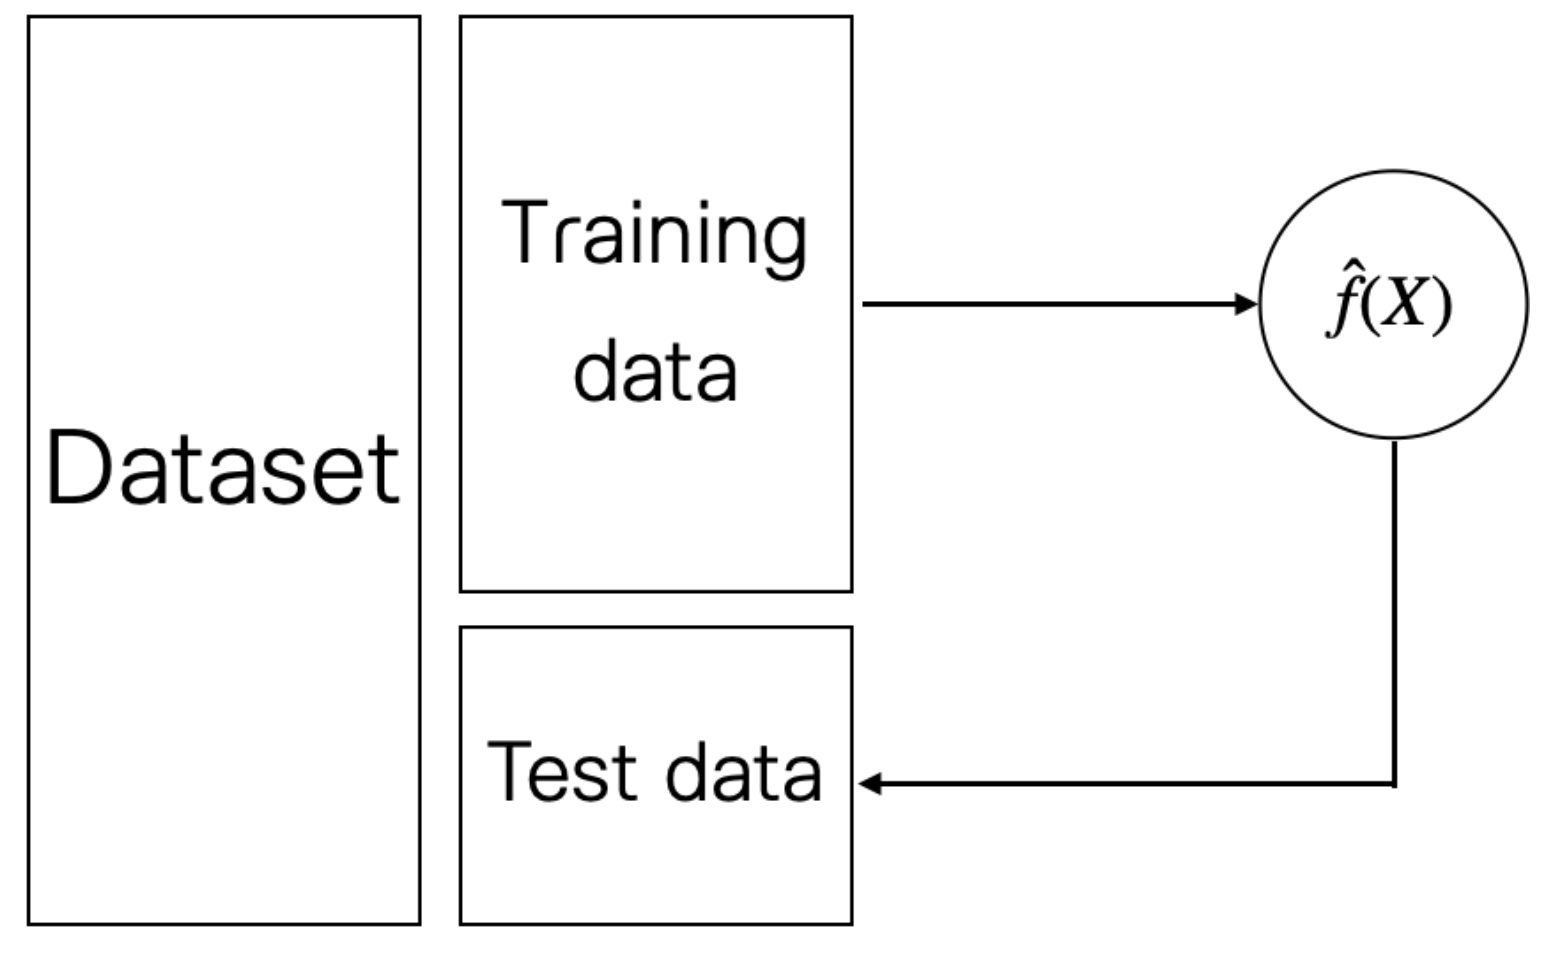
\includegraphics[width=0.5\textwidth,height=\textheight]{/Users/siwachoat/Library/Mobile Documents/com~apple~CloudDocs/github/ssiwacho/2758501/ssiwacho.github.io/2758688/week1/Screen Shot 2563-08-16 at 12.13.22.png}

ตัวอย่างต่อไปนี้แสดงการตรวจสอบประสิทธิภาพของโมเดลโดยใช้ train/test
method ใช้ข้อมูลที่ใช้เป็นตัวอย่างคือชุดข้อมูล state.x77
ที่เก็บรวบรวมข้อมูลอัตราการฆาตกรรม (Murder) กับสภาพทางเศรษฐกิจ สังคม
และภูมิศาสตร์ของแต่ละรัฐในประเทศอเมริกา

\begin{Shaded}
\begin{Highlighting}[]
\NormalTok{dat\textless{}{-}}\KeywordTok{data.frame}\NormalTok{(state.x77) }\CommentTok{\#import and convert data into data.frame}
\KeywordTok{str}\NormalTok{(dat) }\CommentTok{\#exploring dat}
\end{Highlighting}
\end{Shaded}

\begin{verbatim}
## 'data.frame':    50 obs. of  8 variables:
##  $ Population: num  3615 365 2212 2110 21198 ...
##  $ Income    : num  3624 6315 4530 3378 5114 ...
##  $ Illiteracy: num  2.1 1.5 1.8 1.9 1.1 0.7 1.1 0.9 1.3 2 ...
##  $ Life.Exp  : num  69 69.3 70.5 70.7 71.7 ...
##  $ Murder    : num  15.1 11.3 7.8 10.1 10.3 6.8 3.1 6.2 10.7 13.9 ...
##  $ HS.Grad   : num  41.3 66.7 58.1 39.9 62.6 63.9 56 54.6 52.6 40.6 ...
##  $ Frost     : num  20 152 15 65 20 166 139 103 11 60 ...
##  $ Area      : num  50708 566432 113417 51945 156361 ...
\end{verbatim}

\begin{Shaded}
\begin{Highlighting}[]
\KeywordTok{library}\NormalTok{(caret)}
\NormalTok{train.id\textless{}{-}}\KeywordTok{createDataPartition}\NormalTok{(dat}\OperatorTok{$}\NormalTok{Murder,}\DataTypeTok{p=}\FloatTok{0.6}\NormalTok{,}\DataTypeTok{list=}\NormalTok{F) }\CommentTok{\#split the data}
\NormalTok{train.dat\textless{}{-}dat[train.id,] }\CommentTok{\#training dataset}
\NormalTok{test.dat\textless{}{-}dat[}\OperatorTok{{-}}\NormalTok{train.id,] }\CommentTok{\#testing dataset}

\CommentTok{\#trainthe regression model using lm() function}
\NormalTok{fit\textless{}{-}}\KeywordTok{lm}\NormalTok{(Murder}\OperatorTok{\textasciitilde{}}\NormalTok{., }\DataTypeTok{data=}\NormalTok{train.dat)}

\CommentTok{\#calculate predictions and compute performance metric from testing data}
\NormalTok{pred\textless{}{-}}\KeywordTok{predict}\NormalTok{(fit,test.dat)}
\CommentTok{\# plot scatter plot between prediction and real value}
\KeywordTok{plot}\NormalTok{(pred,test.dat}\OperatorTok{$}\NormalTok{Murder,}\DataTypeTok{xlab=}\StringTok{"predicted value"}\NormalTok{,}\DataTypeTok{ylab=}\StringTok{"real observation"}\NormalTok{,}\DataTypeTok{pch=}\DecValTok{16}\NormalTok{)}
\end{Highlighting}
\end{Shaded}

\begin{center}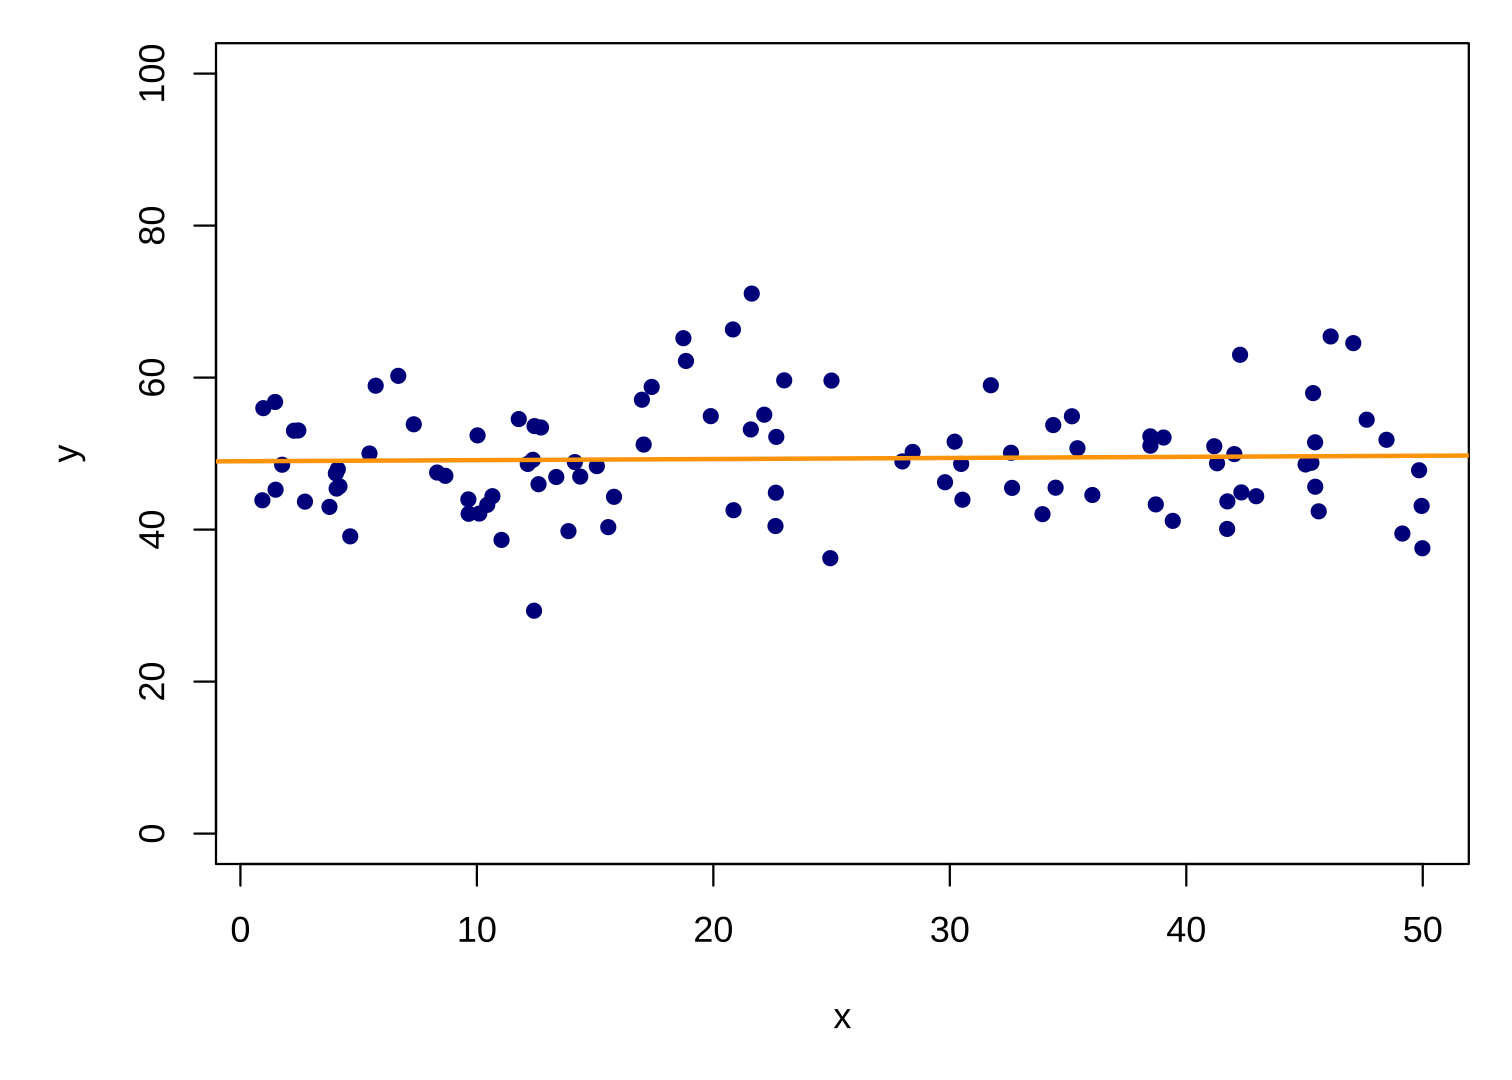
\includegraphics[width=468px]{week3-Model-Evaluation_files/figure-latex/unnamed-chunk-2-1} \end{center}

\textbf{Performance metric}

\begin{Shaded}
\begin{Highlighting}[]
\CommentTok{\# performance metric}
\NormalTok{performance\textless{}{-}}\KeywordTok{data.frame}\NormalTok{(}\KeywordTok{R2}\NormalTok{(pred,test.dat}\OperatorTok{$}\NormalTok{Murder),}
                        \KeywordTok{RMSE}\NormalTok{(pred,test.dat}\OperatorTok{$}\NormalTok{Murder),}
                        \KeywordTok{MAE}\NormalTok{(pred,test.dat}\OperatorTok{$}\NormalTok{Murder))}
\KeywordTok{names}\NormalTok{(performance)\textless{}{-}}\KeywordTok{c}\NormalTok{(}\StringTok{"R2"}\NormalTok{,}\StringTok{"RMSE"}\NormalTok{,}\StringTok{"MAE"}\NormalTok{)}
\NormalTok{performance}
\end{Highlighting}
\end{Shaded}

\begin{verbatim}
##          R2     RMSE      MAE
## 1 0.7050931 2.224173 1.673141
\end{verbatim}

วิธี train/test
เป็นวิธีที่มีประสิทธิภาพดีในกรณีที่ผู้วิเคราะห์มีข้อมูลจำนวนมาก
อย่างไรก็ตามวิธีการนี้ก็มีข้อสังเกตคือ
โมเดลทำนายที่พัฒนาขึ้นพัฒนาจากข้อมูลในชุดข้อมูลฝึกหัดซึ่งเป็นข้อมูลเพียงบางส่วนของข้อมูลทั้งหมด
จึงอาจทำให้โมเดลเกิดความลำเอียงได้ โดยเฉพาะในกรณีที่ข้อมูลมีจำนวนไม่มาก

\textbf{(2) Leave one out cross validation (LOOCV)}
วิธีการนี้แบ่งข้อมูลออกเป็นสองส่วนเช่นเดียวกับวิธีการ train/test
แต่มีความแตกต่างตรงลักษณะของการแบ่ง กล่าวคือวิธีการนี้จะแบ่งข้อมูล 1
ค่าไว้เป็นข้อมูลทดสอบ
จากนั้นใช้ข้อมูลที่เหลือทั้งหมดเพื่อพัฒนาโมเดลสำหรับทำนายข้อมูล 1
ค่าในข้างต้น และเก็บผลประสิทธิภาพการทำนายข้อมูลดังกล่าวไว้
จากนั้นดำเนินกระบวนการข้างต้นซ้ำจนกว่าจะทดสอบข้อมูลครบทุกค่า
และแล้วจึงคำนวณประสิทธิภาพของโมเดลจากค่าประสิทธิภาพการทำนายของข้อมูลที่เก็บไว้

ตัวอย่างต่อไปนี้แสดงการวิเคราะห์ประสิทธิภาพของโมเดลแบบ Leave one out
cross validation โดยใช้ฟังก์ชัน \texttt{train()} ใน package-caret
โดยใช้ข้อมูล \texttt{state.x77} ในข้างต้น

\begin{Shaded}
\begin{Highlighting}[]
\CommentTok{\# specify training control}
\NormalTok{train.clt\textless{}{-}}\KeywordTok{trainControl}\NormalTok{(}\DataTypeTok{method=}\StringTok{"LOOCV"}\NormalTok{)}

\CommentTok{\# train the regression model using train() function}
\NormalTok{fit\textless{}{-}}\KeywordTok{train}\NormalTok{(Murder}\OperatorTok{\textasciitilde{}}\NormalTok{., }\DataTypeTok{data=}\NormalTok{dat,}\DataTypeTok{method=}\StringTok{"lm"}\NormalTok{, }\DataTypeTok{trControl=}\NormalTok{train.clt)}

\CommentTok{\#print the LOOCV results}
\NormalTok{fit}
\end{Highlighting}
\end{Shaded}

\begin{verbatim}
## Linear Regression 
## 
## 50 samples
##  7 predictor
## 
## No pre-processing
## Resampling: Leave-One-Out Cross-Validation 
## Summary of sample sizes: 49, 49, 49, 49, 49, 49, ... 
## Resampling results:
## 
##   RMSE      Rsquared   MAE     
##   2.004621  0.7115175  1.621311
## 
## Tuning parameter 'intercept' was held constant at a value of TRUE
\end{verbatim}

\begin{Shaded}
\begin{Highlighting}[]
\CommentTok{\#regression output}
\KeywordTok{summary}\NormalTok{(fit)}
\end{Highlighting}
\end{Shaded}

\begin{verbatim}
## 
## Call:
## lm(formula = .outcome ~ ., data = dat)
## 
## Residuals:
##     Min      1Q  Median      3Q     Max 
## -3.4452 -1.1016 -0.0598  1.1758  3.2355 
## 
## Coefficients:
##               Estimate Std. Error t value Pr(>|t|)    
## (Intercept)  1.222e+02  1.789e+01   6.831 2.54e-08 ***
## Population   1.880e-04  6.474e-05   2.905  0.00584 ** 
## Income      -1.592e-04  5.725e-04  -0.278  0.78232    
## Illiteracy   1.373e+00  8.322e-01   1.650  0.10641    
## Life.Exp    -1.655e+00  2.562e-01  -6.459 8.68e-08 ***
## HS.Grad      3.234e-02  5.725e-02   0.565  0.57519    
## Frost       -1.288e-02  7.392e-03  -1.743  0.08867 .  
## Area         5.967e-06  3.801e-06   1.570  0.12391    
## ---
## Signif. codes:  0 '***' 0.001 '**' 0.01 '*' 0.05 '.' 0.1 ' ' 1
## 
## Residual standard error: 1.746 on 42 degrees of freedom
## Multiple R-squared:  0.8083, Adjusted R-squared:  0.7763 
## F-statistic: 25.29 on 7 and 42 DF,  p-value: 3.872e-13
\end{verbatim}

วิธี LOOCV มีข้อดีคือโมเดลทำนายถูกพัฒนาข้อมูลทั้งหมดที่มี
จึงทำให้โมเดลทำนายที่ได้มีความลำเอียงต่ำ
อย่างไรก็ตามวิธีการนี้มีข้อจำกัดคือใช้ทรัพยากรในการคำนวณที่ค่อนข้างมาก
โดยเฉพาะในกรณีที่ชุดข้อมูลมีขนาดใหญ่
นอกจากนี้วิธีการนี้ยังมีความไวต่อค่าทำนายที่ผิดปกติอีกด้วย

\textbf{(3) K-fold cross-validation}

วิธีการนี้แตกต่างจาก LOOCV ตรงทีมีการแบ่งชุดข้อมูลออกเป็น k ส่วน
ที่เรียกว่า k-fold จากนั้นเก็บข้อมูล 1
ชุดไว้เพื่อใช้ทดสอบประสิทธิภาพของโมเดล และใช้ชุดข้อมูล k-1
ชุดที่เหลือเพื่อพัฒนาโมเดลทำนายสำหรับทำนายค่าสังเกตในชุดข้อมูลที่เก็บไว้ในข้างต้น
จากนั้นดำเนินกระบวนการข้างต้นซ้ำเพื่อสลับระหว่างชุดข้อมูลทดสอบ
และชุดข้อมูลฝึกหัดจนครบ
แล้วจึงคำนวณค่าประสิทธิภาพของโมเดลจากดัชนีวัดประสิทธิภาพจำนวน k ค่า
รูปต่อไปนี้แสดงกระบวนการ 3-fold cross validation

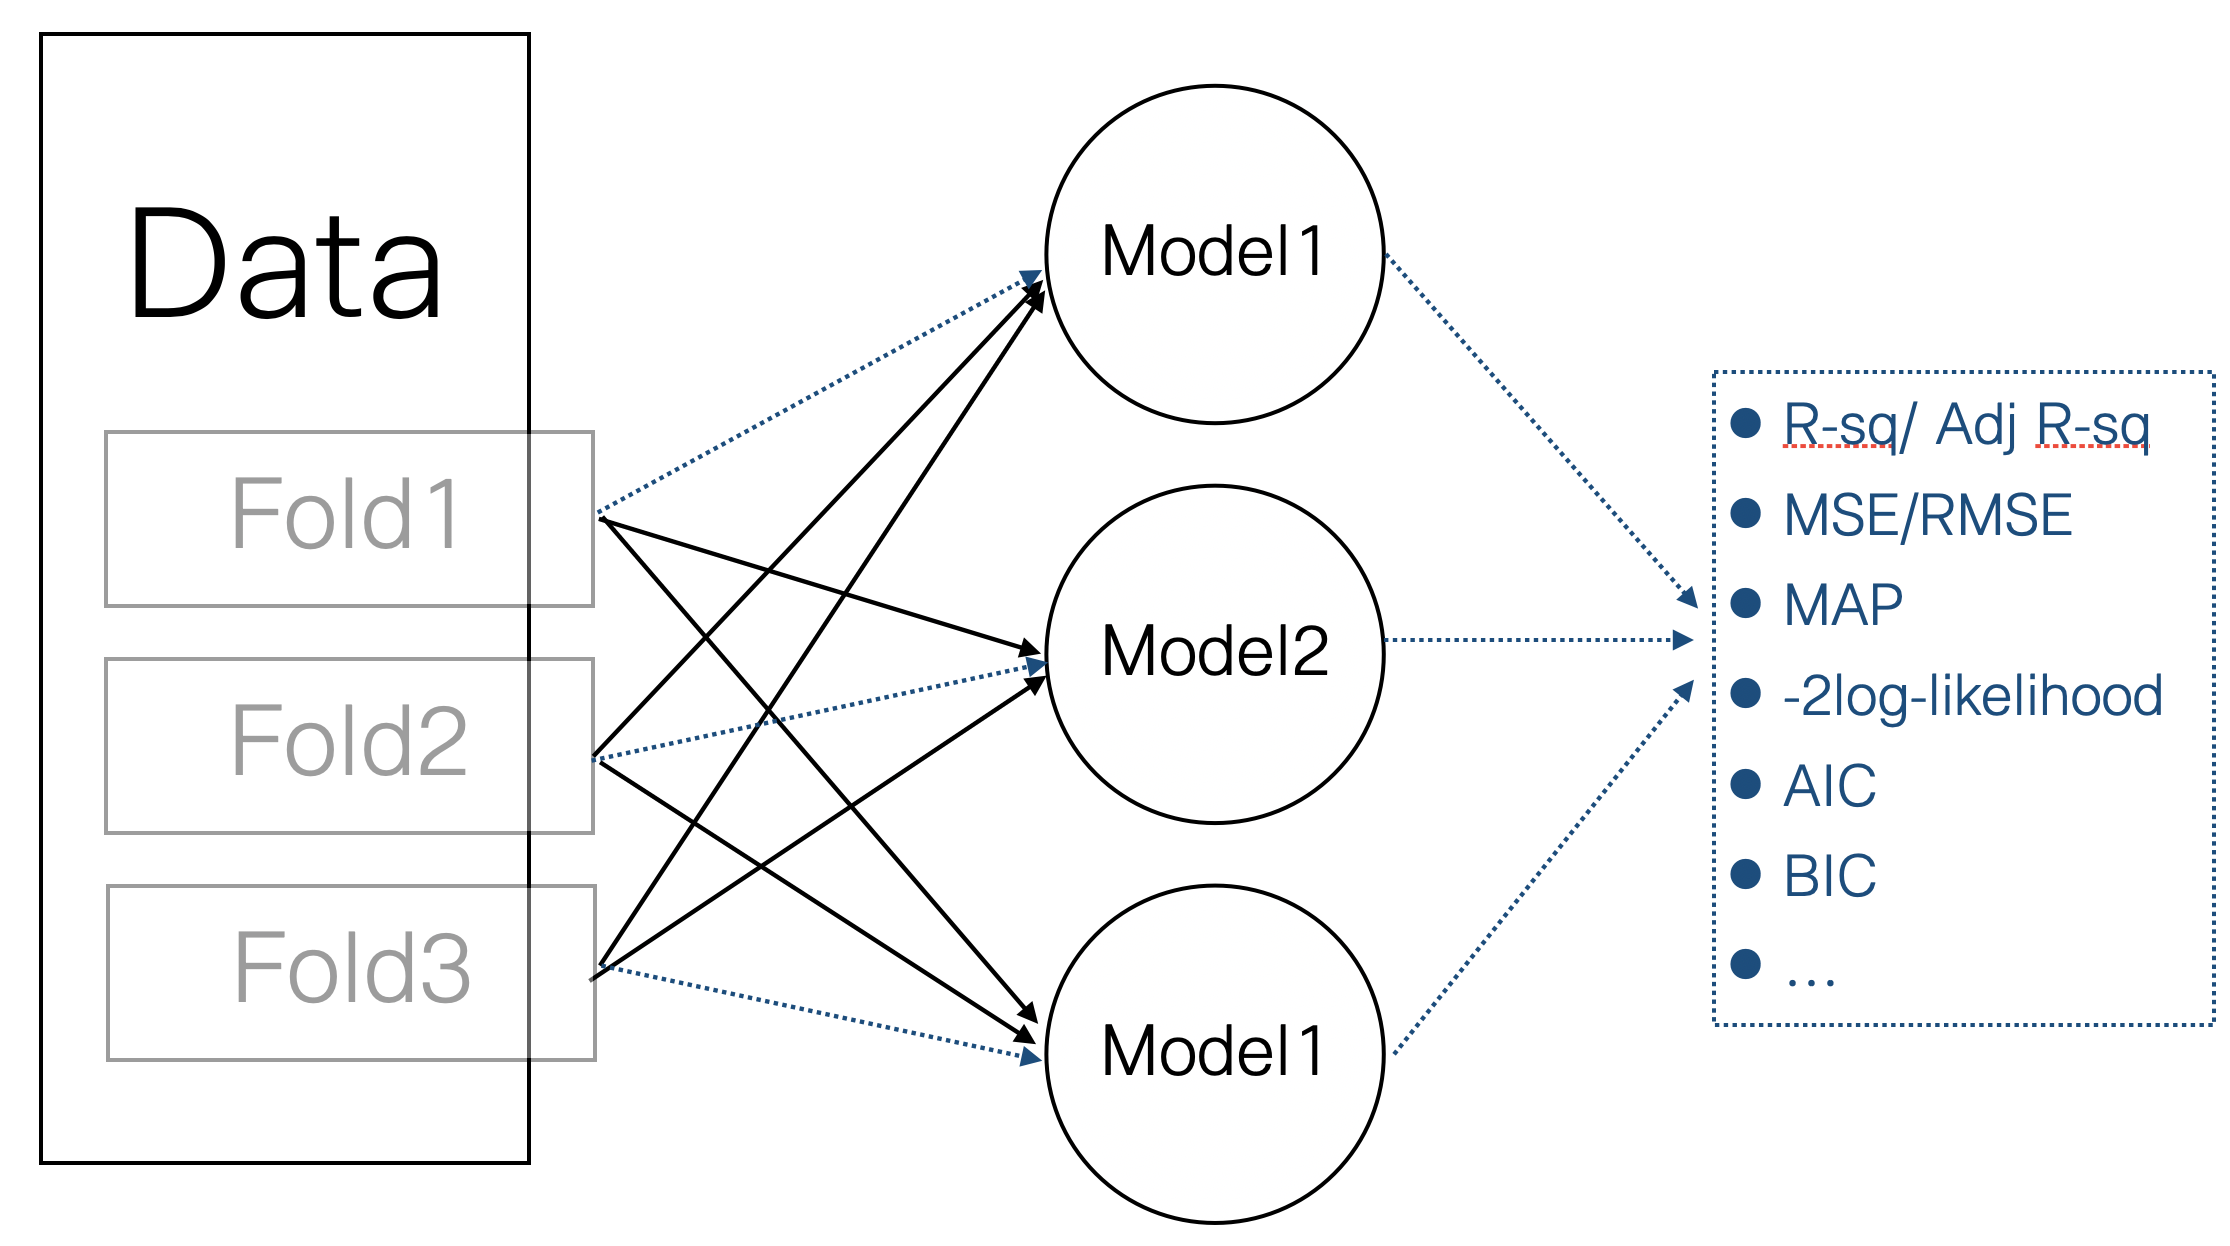
\includegraphics[width=0.7\textwidth,height=\textheight]{/Users/siwachoat/Library/Mobile Documents/com~apple~CloudDocs/github/ssiwacho/2758501/ssiwacho.github.io/2758688/week1/Screen Shot 2563-08-16 at 12.18.04.png}

\begin{Shaded}
\begin{Highlighting}[]
\CommentTok{\# specify the train control}
\NormalTok{train.clt\textless{}{-}}\KeywordTok{trainControl}\NormalTok{(}\DataTypeTok{method=}\StringTok{"cv"}\NormalTok{, }\DataTypeTok{number=}\DecValTok{10}\NormalTok{)}

\CommentTok{\# train the regression model using train() function}
\NormalTok{fit\textless{}{-}}\KeywordTok{train}\NormalTok{(Murder}\OperatorTok{\textasciitilde{}}\NormalTok{., }\DataTypeTok{data=}\NormalTok{dat, }\DataTypeTok{method=}\StringTok{"lm"}\NormalTok{, }\DataTypeTok{trControl=}\NormalTok{train.clt)}

\CommentTok{\# print the CV results}
\NormalTok{fit}
\end{Highlighting}
\end{Shaded}

\begin{verbatim}
## Linear Regression 
## 
## 50 samples
##  7 predictor
## 
## No pre-processing
## Resampling: Cross-Validated (10 fold) 
## Summary of sample sizes: 46, 45, 45, 45, 44, 45, ... 
## Resampling results:
## 
##   RMSE      Rsquared  MAE     
##   1.981908  0.789024  1.635171
## 
## Tuning parameter 'intercept' was held constant at a value of TRUE
\end{verbatim}

วิธีการนี้หากกำหนดให้จำนวน k มีค่ามากขึ้นเรื่อย ๆ
ผลการวิเคราะห์ที่ได้จะมีค่าลู่เข้าหาวิธีการ LOOCV
นอกจากนี้โมเดลทำนายที่ได้จะมีความลำเอียงลดลงตามจำนวน k ที่เพิ่มขึ้น
อย่างไรก็ตามจากการวิจัยที่ผ่านมาพบว่า การกำหนดจำนวน k
ที่เหมาะสมอาจกำหนดให้อยู่ในช่วงตั้งแต่ 5 ถึง 10 (ไม่ได้มีกฎเกณฑ์ตายตัว)
Molinaro (2005) ทำการเปรียบเทียบประสิทธิภาพระหว่างเทคนิค LOOCV กับ
10-fold CV พบว่าให้ผลที่ไม่แตกต่างกัน แต่ประสิทธิภาพในการคำนวณของเทคนิค
CV สามารถทำได้ไวกว่า นอกจากนี้ยังพบว่าการกำหนด k=2 หรือ k=3 ก่อให้เกิด
bias ในการประมาณค่าประสิทธิภาพของโมเดลสูงมาก

\textbf{(4) Repeated K-fold cross-validation}

เทคนิค repeated k-fold CV สามารถใช้เพื่อเสริมประสิทธิภาพให้กับเทคนิค CV
ได้ เทคนิคนี้เป็นการทำ k-fold cross validation ซ้ำได้หลาย ๆ ครั้ง
ซึ่งช่วยลดความลำเอียงของเทคนิค CV ในกรณีที่กำหนดให้ k มีจำนวนน้อย ๆ

\begin{Shaded}
\begin{Highlighting}[]
\NormalTok{train.clt\textless{}{-}}\KeywordTok{trainControl}\NormalTok{(}\DataTypeTok{method=}\StringTok{"repeatedcv"}\NormalTok{, }\DataTypeTok{number=}\DecValTok{5}\NormalTok{, }\DataTypeTok{repeats=}\DecValTok{5}\NormalTok{)}
\NormalTok{fit\textless{}{-}}\KeywordTok{train}\NormalTok{(Murder}\OperatorTok{\textasciitilde{}}\NormalTok{., }\DataTypeTok{data=}\NormalTok{dat, }\DataTypeTok{method=}\StringTok{"lm"}\NormalTok{, }\DataTypeTok{trControl=}\NormalTok{train.clt)}
\NormalTok{fit}
\end{Highlighting}
\end{Shaded}

\begin{verbatim}
## Linear Regression 
## 
## 50 samples
##  7 predictor
## 
## No pre-processing
## Resampling: Cross-Validated (5 fold, repeated 5 times) 
## Summary of sample sizes: 40, 40, 39, 41, 40, 39, ... 
## Resampling results:
## 
##   RMSE     Rsquared   MAE     
##   2.03859  0.7389092  1.689879
## 
## Tuning parameter 'intercept' was held constant at a value of TRUE
\end{verbatim}

\end{document}
